%Autor: Simon Walker
%Version: 1.0
%Datum: 25.11.2019
%Lizenz: CC BY-NC-SA

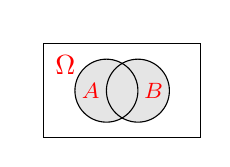
\begin{tikzpicture}[xscale=0.4, yscale=0.4]
	\fill[white, fill opacity=0] (-0.5,0) rectangle (5, 3.5); % Weisser rand um Grafik
	
	%\fill[white] (0,0) rectangle (5,3);
	\draw (0,0) rectangle (5,3);
	\node[red] at (0.7,2.3) {$\Omega$};
	
	\fill[gray!20] (2,1.5) circle[radius=1]; %Fläche färben
	\fill[gray!20] (3,1.5) circle[radius=1];
	
	\draw (2,1.5) circle[radius=1]; %Kreise Zeichnen
	\draw (3,1.5) circle[radius=1];
	
	\node[red] at (1.5, 1.5) {\footnotesize$A$};
	\node[red] at (3.5, 1.5) {\footnotesize$B$};
	
	%\draw[help lines] (0,0) grid (5,3);
\end{tikzpicture}
